\chapter{Data Analysis}
This project will investigate if there exists a cointegrating relation between the four cryptocurrencies namely, Bitcoin, Ethereum, Solana and Ripple. In this chapter, we will examine the data with visual interpretation of plots and qualitative tests.

\section{Data Introduction}
The data that has been used can be found [ref].\\




\begin{figure}[!ht]
  \centering
  \subfloat[][]{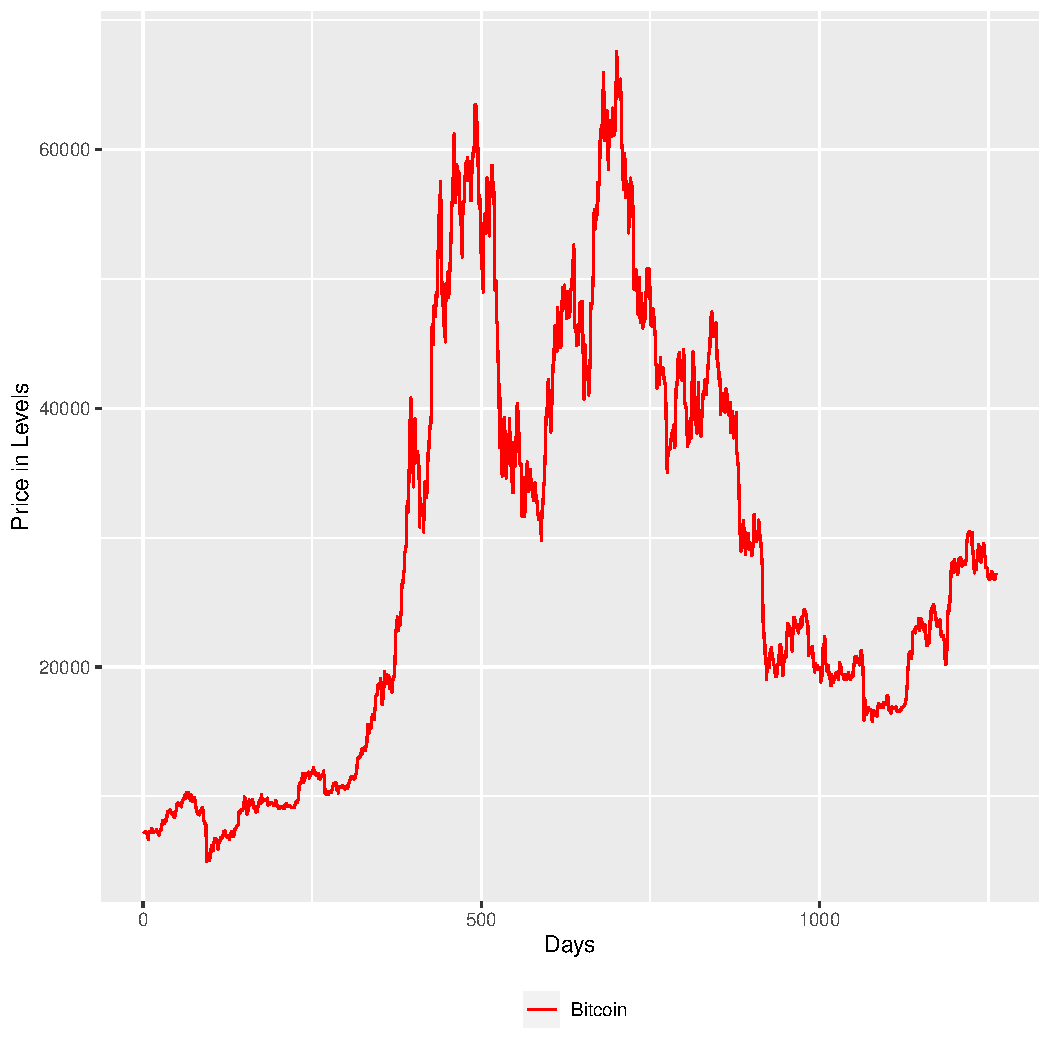
\includegraphics[width=.45\textwidth]{1.Projekt_kode/Billeder/Crypto_in_levels_Bitcoin.pdf}}\quad
  \subfloat[][]{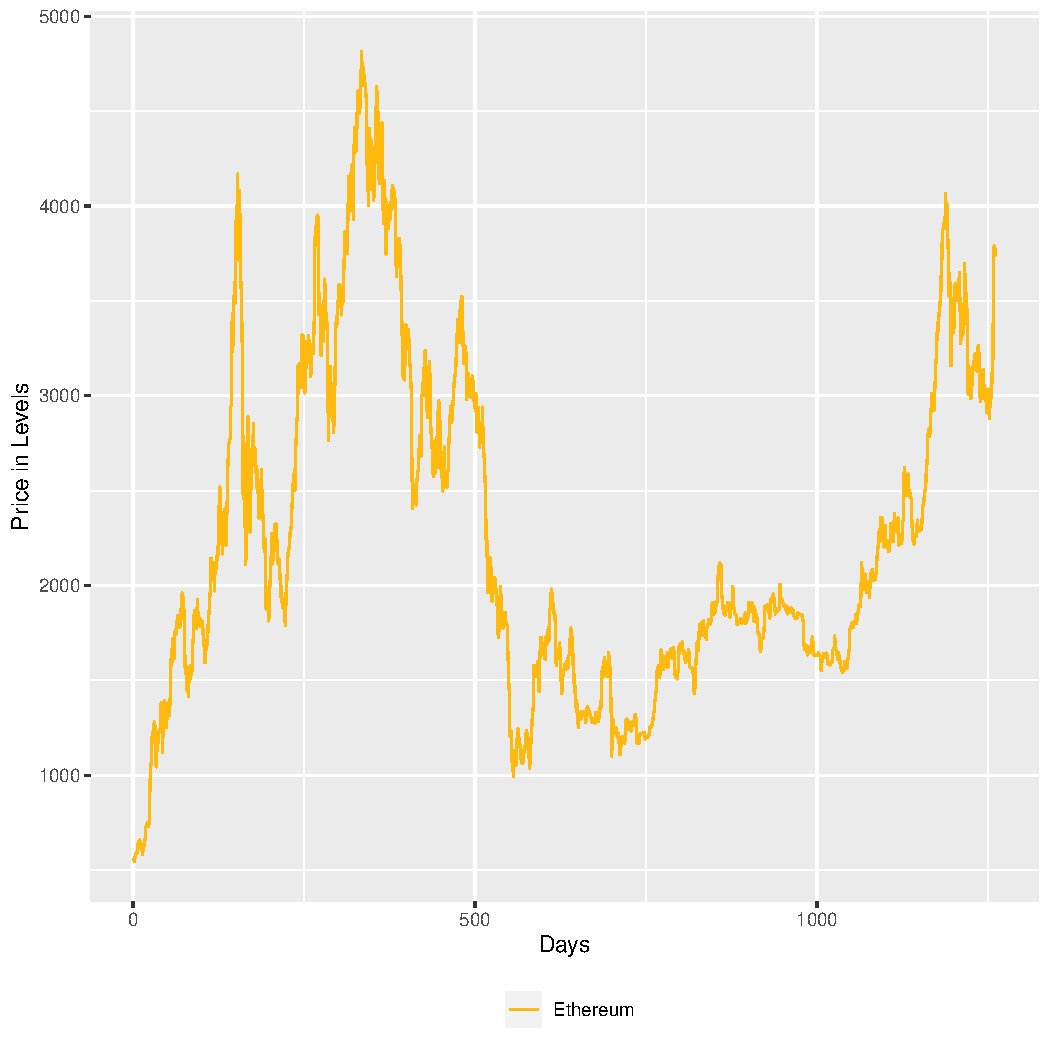
\includegraphics[width=.45\textwidth]{1.Projekt_kode/Billeder/Crypto_in_levels_Ethereum.pdf}}\\
  \subfloat[][]{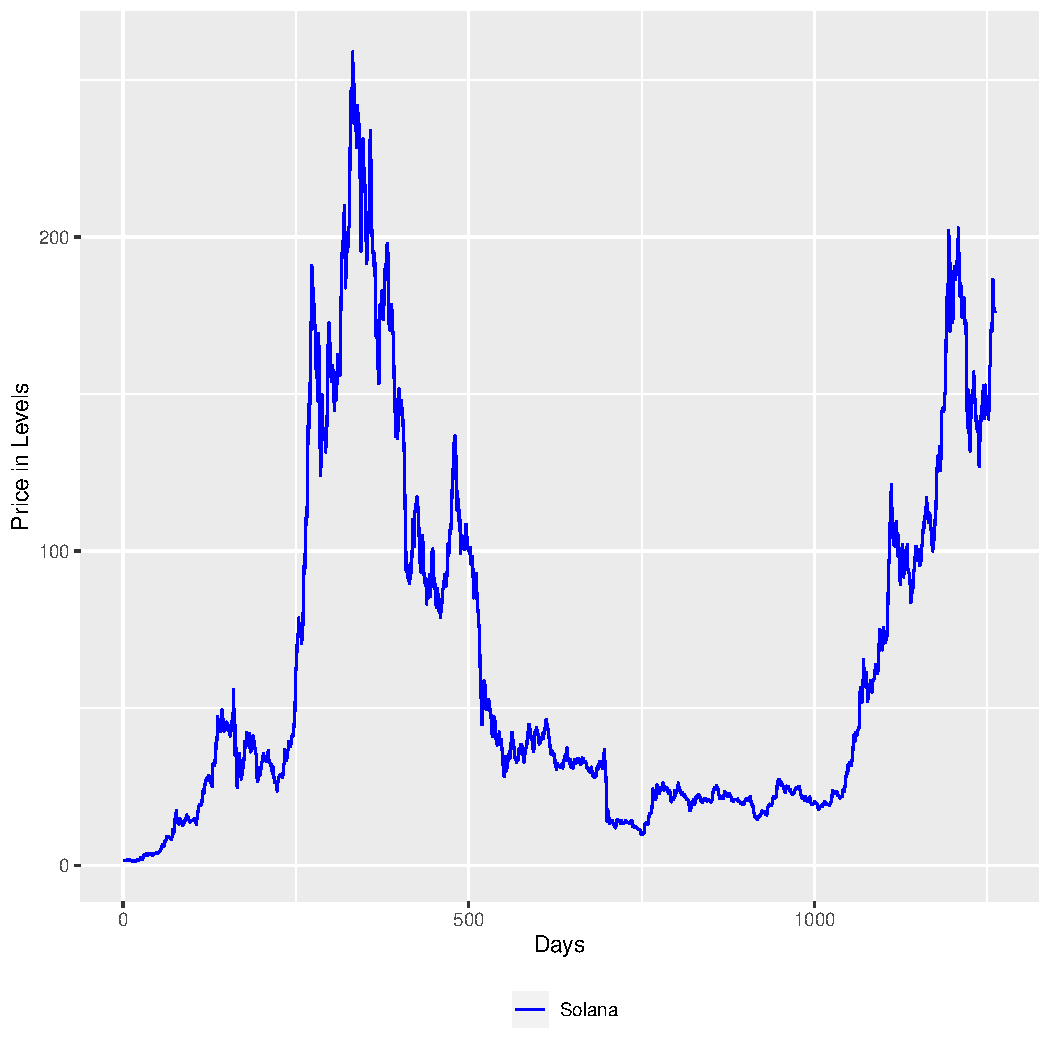
\includegraphics[width=.45\textwidth]{1.Projekt_kode/Billeder/Crypto_in_levels_Solana.pdf}}\quad
  \subfloat[][]{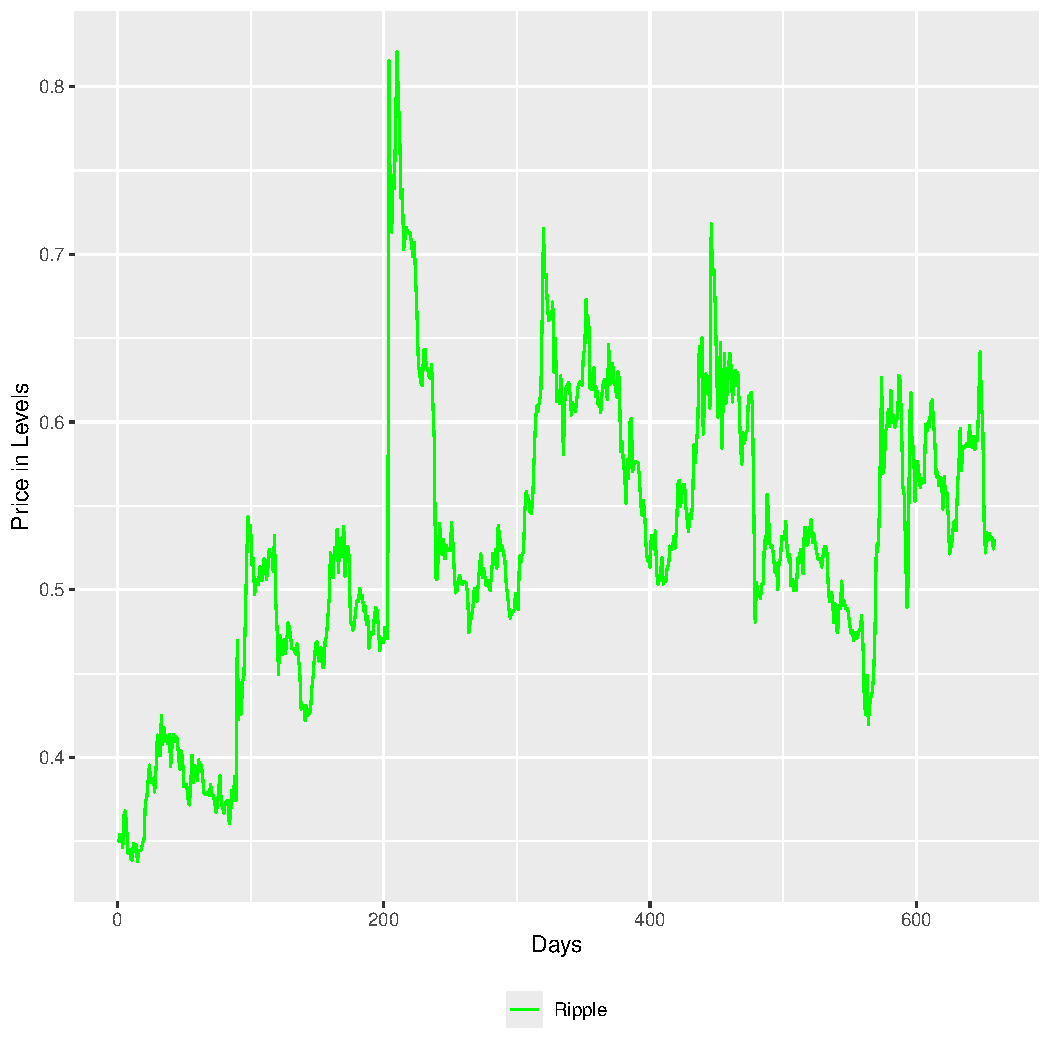
\includegraphics[width=.45\textwidth]{1.Projekt_kode/Billeder/Crypto_in_levels_Ripple.pdf}}
  \caption{First group of subfigures.}
  \label{fig:sub1}
\end{figure}
A visual inspection of the data in levels reveal no trend
\newpage
Number of lags in our model
\begin{figure}
    \centering
    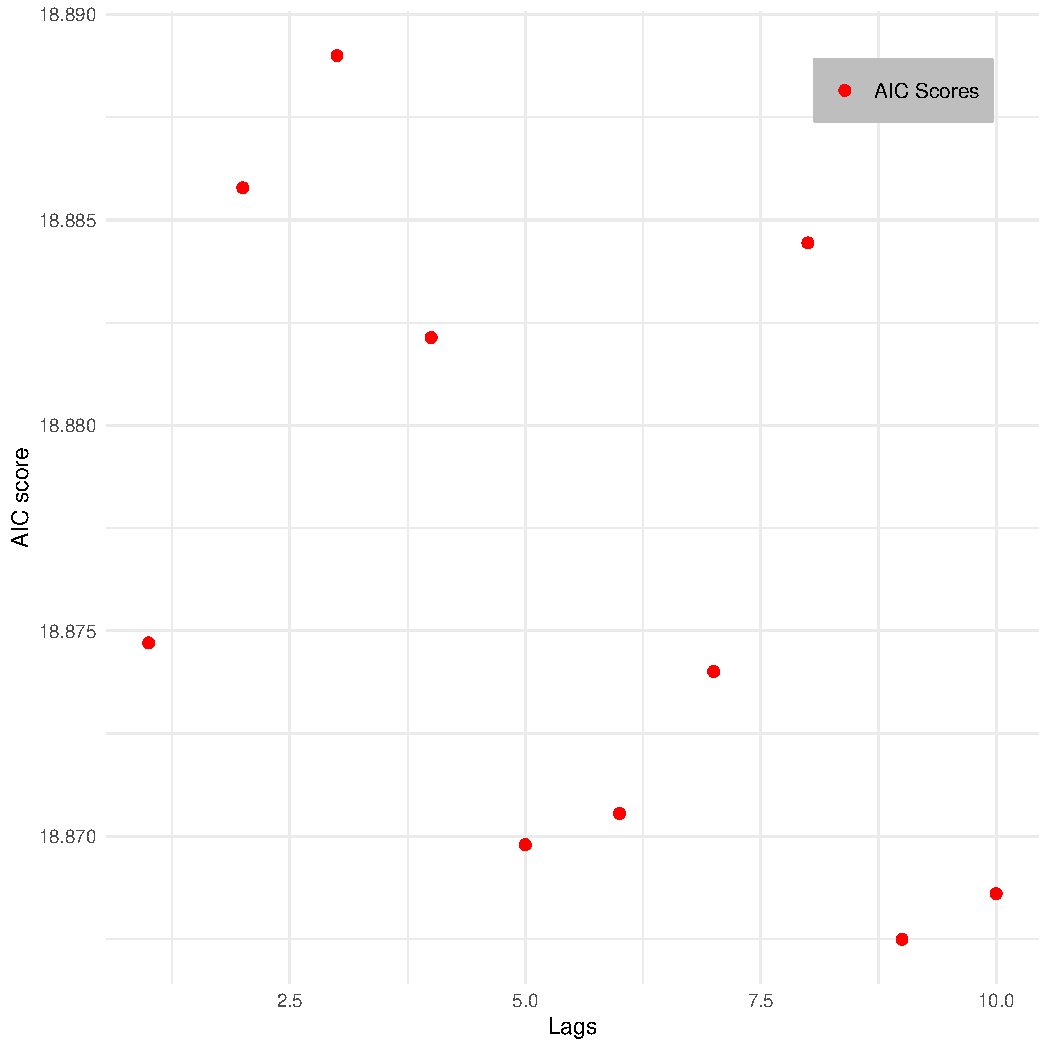
\includegraphics[width=0.5\linewidth]{1.Projekt_kode/Billeder/Crypto_lags.pdf}
    \caption{AIC score for different lags}
    \label{fig:enter-label}
\end{figure}

residuals acf og histogram

\begin{figure}[!ht]
  \centering
  \subfloat[][]{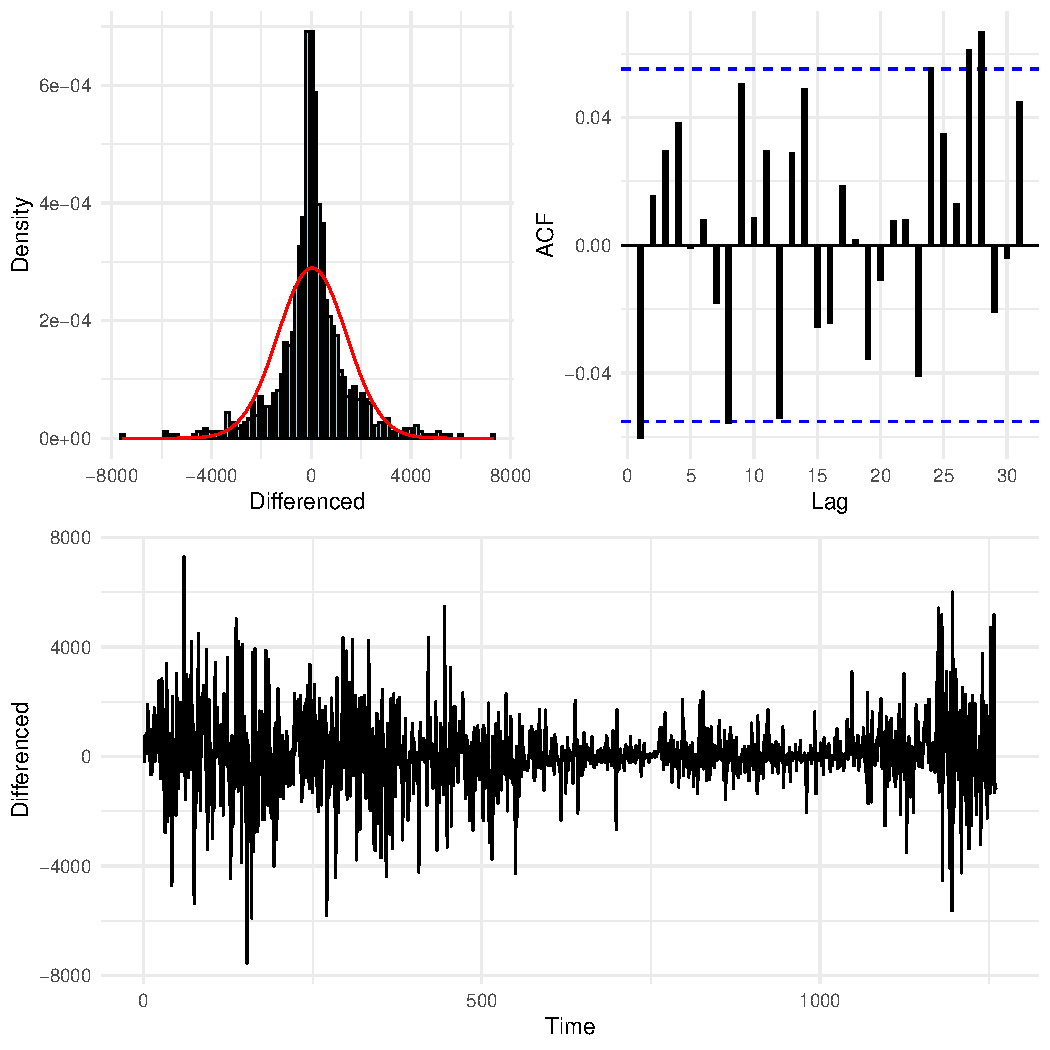
\includegraphics[width=.45\textwidth]{1.Projekt_kode/Billeder/plot_grid_Bitcoin.pdf}}\quad
  \subfloat[][]{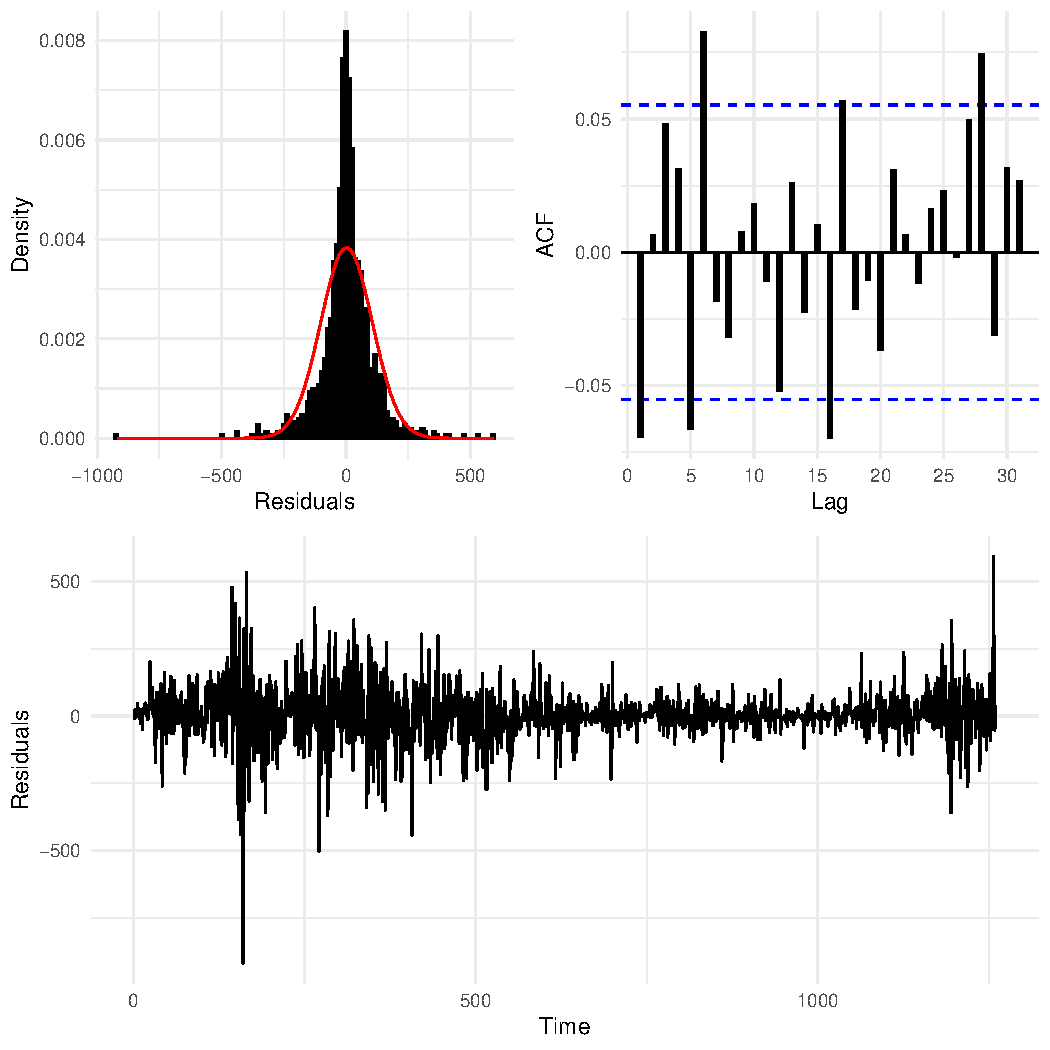
\includegraphics[width=.45\textwidth]{1.Projekt_kode/Billeder/plot_grid_Ethereum.pdf}}\\
  \subfloat[][]{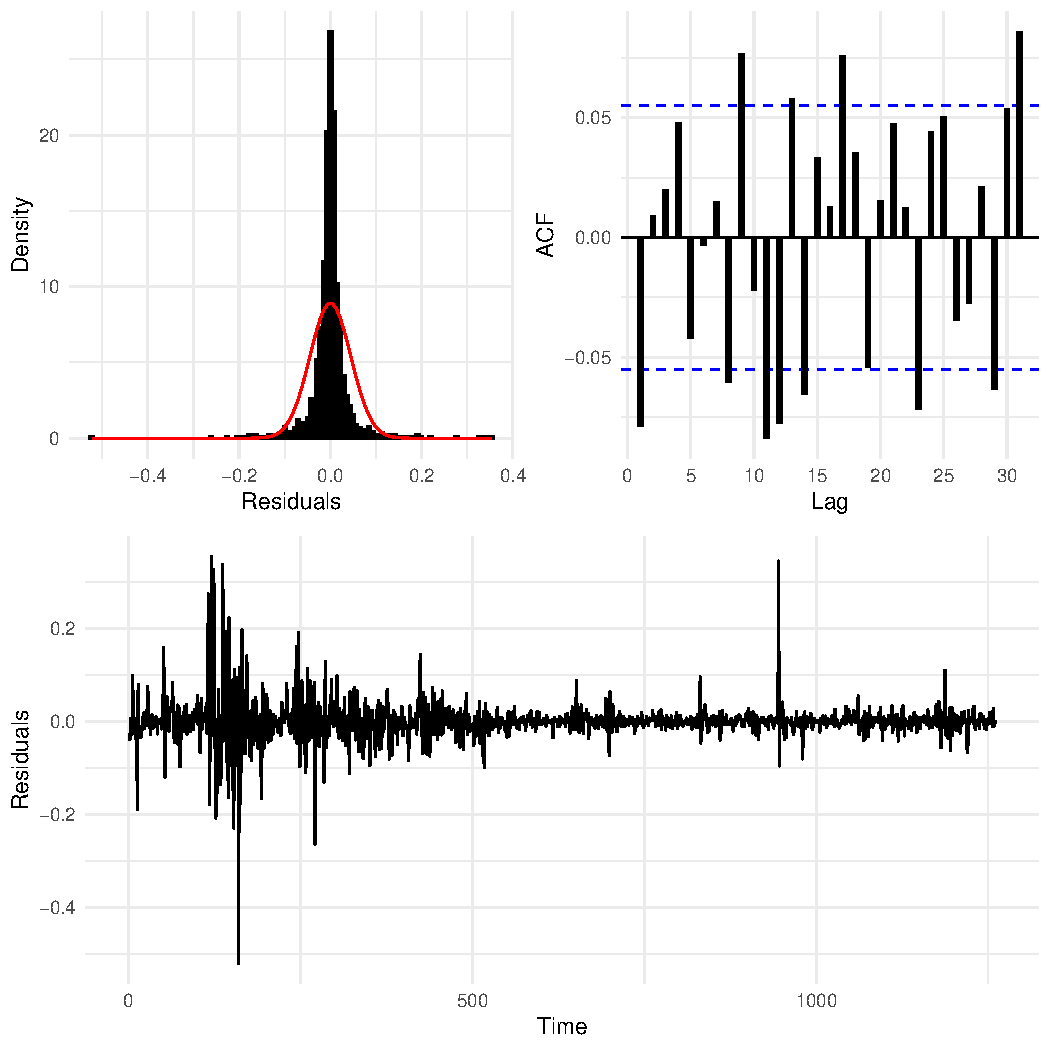
\includegraphics[width=.45\textwidth]{1.Projekt_kode/Billeder/plot_grid_Ripple.pdf}}\quad
  \subfloat[][]{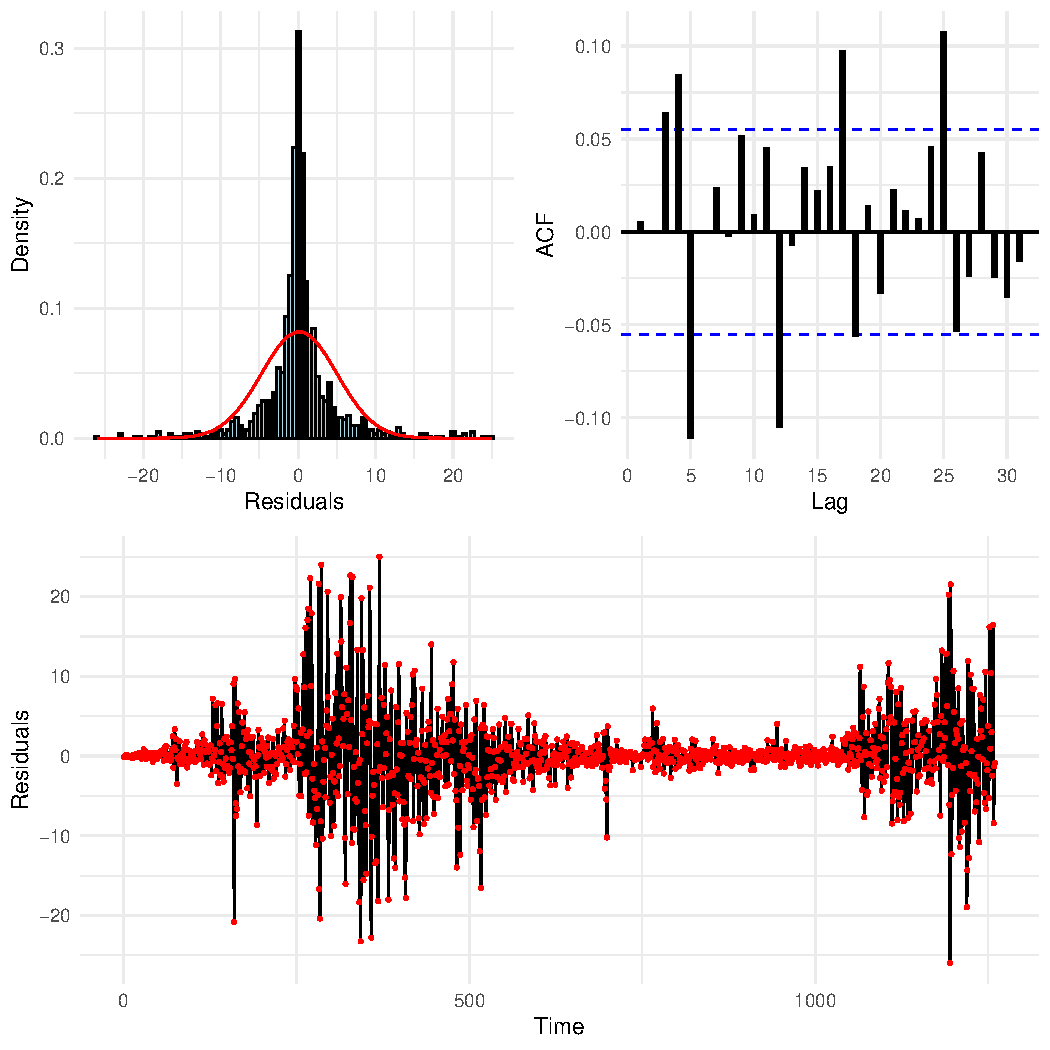
\includegraphics[width=.45\textwidth]{1.Projekt_kode/Billeder/plot_grid_Solana.pdf}}
  \caption{First group of subfigures.}
  \label{fig:sub1}
\end{figure}
